


% Header, overrides base

    % Make sure that the sphinx doc style knows who it inherits from.
    \def\sphinxdocclass{article}

    % Declare the document class
    \documentclass[letterpaper,10pt,english]{/usr/lib/python3.3/site-packages/sphinx/texinputs/sphinxhowto}

    % Imports
    \usepackage[utf8]{inputenc}
    \DeclareUnicodeCharacter{00A0}{\\nobreakspace}
    \usepackage[T1]{fontenc}
    \usepackage{babel}
    \usepackage{times}
    \usepackage{import}
    \usepackage[Bjarne]{/usr/lib/python3.3/site-packages/sphinx/texinputs/fncychap}
    \usepackage{longtable}
    \usepackage{/usr/lib/python3.3/site-packages/sphinx/texinputs/sphinx}
    \usepackage{multirow}

    \usepackage{amsmath}
    \usepackage{amssymb}
    \usepackage{ucs}
    \usepackage{enumerate}

    % Used to make the Input/Output rules follow around the contents.
    \usepackage{needspace}

    % Pygments requirements
    \usepackage{fancyvrb}
    \usepackage{color}
    % ansi colors additions
    \definecolor{darkgreen}{rgb}{.12,.54,.11}
    \definecolor{lightgray}{gray}{.95}
    \definecolor{brown}{rgb}{0.54,0.27,0.07}
    \definecolor{purple}{rgb}{0.5,0.0,0.5}
    \definecolor{darkgray}{gray}{0.25}
    \definecolor{lightred}{rgb}{1.0,0.39,0.28}
    \definecolor{lightgreen}{rgb}{0.48,0.99,0.0}
    \definecolor{lightblue}{rgb}{0.53,0.81,0.92}
    \definecolor{lightpurple}{rgb}{0.87,0.63,0.87}
    \definecolor{lightcyan}{rgb}{0.5,1.0,0.83}

    % Needed to box output/input
    \usepackage{tikz}
        \usetikzlibrary{calc,arrows,shadows}
    \usepackage[framemethod=tikz]{mdframed}

    \usepackage{alltt}

    % Used to load and display graphics
    \usepackage{graphicx}
    \graphicspath{ {figs/} }
    \usepackage[Export]{adjustbox} % To resize

    % used so that images for notebooks which have spaces in the name can still be included
    \usepackage{grffile}


    % For formatting output while also word wrapping.
    \usepackage{listings}
    \lstset{breaklines=true}
    \lstset{basicstyle=\small\ttfamily}
    \def\smaller{\fontsize{9.5pt}{9.5pt}\selectfont}

    %Pygments definitions
    
\makeatletter
\def\PY@reset{\let\PY@it=\relax \let\PY@bf=\relax%
    \let\PY@ul=\relax \let\PY@tc=\relax%
    \let\PY@bc=\relax \let\PY@ff=\relax}
\def\PY@tok#1{\csname PY@tok@#1\endcsname}
\def\PY@toks#1+{\ifx\relax#1\empty\else%
    \PY@tok{#1}\expandafter\PY@toks\fi}
\def\PY@do#1{\PY@bc{\PY@tc{\PY@ul{%
    \PY@it{\PY@bf{\PY@ff{#1}}}}}}}
\def\PY#1#2{\PY@reset\PY@toks#1+\relax+\PY@do{#2}}

\expandafter\def\csname PY@tok@bp\endcsname{\def\PY@tc##1{\textcolor[rgb]{0.00,0.50,0.00}{##1}}}
\expandafter\def\csname PY@tok@se\endcsname{\let\PY@bf=\textbf\def\PY@tc##1{\textcolor[rgb]{0.73,0.40,0.13}{##1}}}
\expandafter\def\csname PY@tok@sd\endcsname{\let\PY@it=\textit\def\PY@tc##1{\textcolor[rgb]{0.73,0.13,0.13}{##1}}}
\expandafter\def\csname PY@tok@sc\endcsname{\def\PY@tc##1{\textcolor[rgb]{0.73,0.13,0.13}{##1}}}
\expandafter\def\csname PY@tok@sb\endcsname{\def\PY@tc##1{\textcolor[rgb]{0.73,0.13,0.13}{##1}}}
\expandafter\def\csname PY@tok@c1\endcsname{\let\PY@it=\textit\def\PY@tc##1{\textcolor[rgb]{0.25,0.50,0.50}{##1}}}
\expandafter\def\csname PY@tok@nt\endcsname{\let\PY@bf=\textbf\def\PY@tc##1{\textcolor[rgb]{0.00,0.50,0.00}{##1}}}
\expandafter\def\csname PY@tok@nv\endcsname{\def\PY@tc##1{\textcolor[rgb]{0.10,0.09,0.49}{##1}}}
\expandafter\def\csname PY@tok@err\endcsname{\def\PY@bc##1{\setlength{\fboxsep}{0pt}\fcolorbox[rgb]{1.00,0.00,0.00}{1,1,1}{\strut ##1}}}
\expandafter\def\csname PY@tok@si\endcsname{\let\PY@bf=\textbf\def\PY@tc##1{\textcolor[rgb]{0.73,0.40,0.53}{##1}}}
\expandafter\def\csname PY@tok@sh\endcsname{\def\PY@tc##1{\textcolor[rgb]{0.73,0.13,0.13}{##1}}}
\expandafter\def\csname PY@tok@nl\endcsname{\def\PY@tc##1{\textcolor[rgb]{0.63,0.63,0.00}{##1}}}
\expandafter\def\csname PY@tok@nn\endcsname{\let\PY@bf=\textbf\def\PY@tc##1{\textcolor[rgb]{0.00,0.00,1.00}{##1}}}
\expandafter\def\csname PY@tok@no\endcsname{\def\PY@tc##1{\textcolor[rgb]{0.53,0.00,0.00}{##1}}}
\expandafter\def\csname PY@tok@ss\endcsname{\def\PY@tc##1{\textcolor[rgb]{0.10,0.09,0.49}{##1}}}
\expandafter\def\csname PY@tok@ni\endcsname{\let\PY@bf=\textbf\def\PY@tc##1{\textcolor[rgb]{0.60,0.60,0.60}{##1}}}
\expandafter\def\csname PY@tok@nd\endcsname{\def\PY@tc##1{\textcolor[rgb]{0.67,0.13,1.00}{##1}}}
\expandafter\def\csname PY@tok@ne\endcsname{\let\PY@bf=\textbf\def\PY@tc##1{\textcolor[rgb]{0.82,0.25,0.23}{##1}}}
\expandafter\def\csname PY@tok@nf\endcsname{\def\PY@tc##1{\textcolor[rgb]{0.00,0.00,1.00}{##1}}}
\expandafter\def\csname PY@tok@na\endcsname{\def\PY@tc##1{\textcolor[rgb]{0.49,0.56,0.16}{##1}}}
\expandafter\def\csname PY@tok@nb\endcsname{\def\PY@tc##1{\textcolor[rgb]{0.00,0.50,0.00}{##1}}}
\expandafter\def\csname PY@tok@nc\endcsname{\let\PY@bf=\textbf\def\PY@tc##1{\textcolor[rgb]{0.00,0.00,1.00}{##1}}}
\expandafter\def\csname PY@tok@kn\endcsname{\let\PY@bf=\textbf\def\PY@tc##1{\textcolor[rgb]{0.00,0.50,0.00}{##1}}}
\expandafter\def\csname PY@tok@c\endcsname{\let\PY@it=\textit\def\PY@tc##1{\textcolor[rgb]{0.25,0.50,0.50}{##1}}}
\expandafter\def\csname PY@tok@m\endcsname{\def\PY@tc##1{\textcolor[rgb]{0.40,0.40,0.40}{##1}}}
\expandafter\def\csname PY@tok@il\endcsname{\def\PY@tc##1{\textcolor[rgb]{0.40,0.40,0.40}{##1}}}
\expandafter\def\csname PY@tok@o\endcsname{\def\PY@tc##1{\textcolor[rgb]{0.40,0.40,0.40}{##1}}}
\expandafter\def\csname PY@tok@kd\endcsname{\let\PY@bf=\textbf\def\PY@tc##1{\textcolor[rgb]{0.00,0.50,0.00}{##1}}}
\expandafter\def\csname PY@tok@kc\endcsname{\let\PY@bf=\textbf\def\PY@tc##1{\textcolor[rgb]{0.00,0.50,0.00}{##1}}}
\expandafter\def\csname PY@tok@k\endcsname{\let\PY@bf=\textbf\def\PY@tc##1{\textcolor[rgb]{0.00,0.50,0.00}{##1}}}
\expandafter\def\csname PY@tok@w\endcsname{\def\PY@tc##1{\textcolor[rgb]{0.73,0.73,0.73}{##1}}}
\expandafter\def\csname PY@tok@ow\endcsname{\let\PY@bf=\textbf\def\PY@tc##1{\textcolor[rgb]{0.67,0.13,1.00}{##1}}}
\expandafter\def\csname PY@tok@s\endcsname{\def\PY@tc##1{\textcolor[rgb]{0.73,0.13,0.13}{##1}}}
\expandafter\def\csname PY@tok@kt\endcsname{\def\PY@tc##1{\textcolor[rgb]{0.69,0.00,0.25}{##1}}}
\expandafter\def\csname PY@tok@kr\endcsname{\let\PY@bf=\textbf\def\PY@tc##1{\textcolor[rgb]{0.00,0.50,0.00}{##1}}}
\expandafter\def\csname PY@tok@kp\endcsname{\def\PY@tc##1{\textcolor[rgb]{0.00,0.50,0.00}{##1}}}
\expandafter\def\csname PY@tok@gi\endcsname{\def\PY@tc##1{\textcolor[rgb]{0.00,0.63,0.00}{##1}}}
\expandafter\def\csname PY@tok@gh\endcsname{\let\PY@bf=\textbf\def\PY@tc##1{\textcolor[rgb]{0.00,0.00,0.50}{##1}}}
\expandafter\def\csname PY@tok@go\endcsname{\def\PY@tc##1{\textcolor[rgb]{0.53,0.53,0.53}{##1}}}
\expandafter\def\csname PY@tok@cp\endcsname{\def\PY@tc##1{\textcolor[rgb]{0.74,0.48,0.00}{##1}}}
\expandafter\def\csname PY@tok@cs\endcsname{\let\PY@it=\textit\def\PY@tc##1{\textcolor[rgb]{0.25,0.50,0.50}{##1}}}
\expandafter\def\csname PY@tok@ge\endcsname{\let\PY@it=\textit}
\expandafter\def\csname PY@tok@gd\endcsname{\def\PY@tc##1{\textcolor[rgb]{0.63,0.00,0.00}{##1}}}
\expandafter\def\csname PY@tok@mi\endcsname{\def\PY@tc##1{\textcolor[rgb]{0.40,0.40,0.40}{##1}}}
\expandafter\def\csname PY@tok@mh\endcsname{\def\PY@tc##1{\textcolor[rgb]{0.40,0.40,0.40}{##1}}}
\expandafter\def\csname PY@tok@s2\endcsname{\def\PY@tc##1{\textcolor[rgb]{0.73,0.13,0.13}{##1}}}
\expandafter\def\csname PY@tok@s1\endcsname{\def\PY@tc##1{\textcolor[rgb]{0.73,0.13,0.13}{##1}}}
\expandafter\def\csname PY@tok@gs\endcsname{\let\PY@bf=\textbf}
\expandafter\def\csname PY@tok@gr\endcsname{\def\PY@tc##1{\textcolor[rgb]{1.00,0.00,0.00}{##1}}}
\expandafter\def\csname PY@tok@cm\endcsname{\let\PY@it=\textit\def\PY@tc##1{\textcolor[rgb]{0.25,0.50,0.50}{##1}}}
\expandafter\def\csname PY@tok@gp\endcsname{\let\PY@bf=\textbf\def\PY@tc##1{\textcolor[rgb]{0.00,0.00,0.50}{##1}}}
\expandafter\def\csname PY@tok@gu\endcsname{\let\PY@bf=\textbf\def\PY@tc##1{\textcolor[rgb]{0.50,0.00,0.50}{##1}}}
\expandafter\def\csname PY@tok@gt\endcsname{\def\PY@tc##1{\textcolor[rgb]{0.00,0.27,0.87}{##1}}}
\expandafter\def\csname PY@tok@mo\endcsname{\def\PY@tc##1{\textcolor[rgb]{0.40,0.40,0.40}{##1}}}
\expandafter\def\csname PY@tok@vg\endcsname{\def\PY@tc##1{\textcolor[rgb]{0.10,0.09,0.49}{##1}}}
\expandafter\def\csname PY@tok@vc\endcsname{\def\PY@tc##1{\textcolor[rgb]{0.10,0.09,0.49}{##1}}}
\expandafter\def\csname PY@tok@sx\endcsname{\def\PY@tc##1{\textcolor[rgb]{0.00,0.50,0.00}{##1}}}
\expandafter\def\csname PY@tok@vi\endcsname{\def\PY@tc##1{\textcolor[rgb]{0.10,0.09,0.49}{##1}}}
\expandafter\def\csname PY@tok@mf\endcsname{\def\PY@tc##1{\textcolor[rgb]{0.40,0.40,0.40}{##1}}}
\expandafter\def\csname PY@tok@sr\endcsname{\def\PY@tc##1{\textcolor[rgb]{0.73,0.40,0.53}{##1}}}

\def\PYZbs{\char`\\}
\def\PYZus{\char`\_}
\def\PYZob{\char`\{}
\def\PYZcb{\char`\}}
\def\PYZca{\char`\^}
\def\PYZam{\char`\&}
\def\PYZlt{\char`\<}
\def\PYZgt{\char`\>}
\def\PYZsh{\char`\#}
\def\PYZpc{\char`\%}
\def\PYZdl{\char`\$}
\def\PYZhy{\char`\-}
\def\PYZsq{\char`\'}
\def\PYZdq{\char`\"}
\def\PYZti{\char`\~}
% for compatibility with earlier versions
\def\PYZat{@}
\def\PYZlb{[}
\def\PYZrb{]}
\makeatother


    %Set pygments styles if needed...
    
        \definecolor{nbframe-border}{rgb}{0.867,0.867,0.867}
        \definecolor{nbframe-bg}{rgb}{0.969,0.969,0.969}
        \definecolor{nbframe-in-prompt}{rgb}{0.0,0.0,0.502}
        \definecolor{nbframe-out-prompt}{rgb}{0.545,0.0,0.0}

        \newenvironment{ColorVerbatim}
        {\begin{mdframed}[%
            roundcorner=1.0pt, %
            backgroundcolor=nbframe-bg, %
            userdefinedwidth=1\linewidth, %
            leftmargin=0.1\linewidth, %
            innerleftmargin=0pt, %
            innerrightmargin=0pt, %
            linecolor=nbframe-border, %
            linewidth=1pt, %
            usetwoside=false, %
            everyline=true, %
            innerlinewidth=3pt, %
            innerlinecolor=nbframe-bg, %
            middlelinewidth=1pt, %
            middlelinecolor=nbframe-bg, %
            outerlinewidth=0.5pt, %
            outerlinecolor=nbframe-border, %
            needspace=0pt
        ]}
        {\end{mdframed}}
        
        \newenvironment{InvisibleVerbatim}
        {\begin{mdframed}[leftmargin=0.1\linewidth,innerleftmargin=3pt,innerrightmargin=3pt, userdefinedwidth=1\linewidth, linewidth=0pt, linecolor=white, usetwoside=false]}
        {\end{mdframed}}

        \renewenvironment{Verbatim}[1][\unskip]
        {\begin{alltt}\smaller}
        {\end{alltt}}
    

    % Help prevent overflowing lines due to urls and other hard-to-break 
    % entities.  This doesn't catch everything...
    \sloppy

    % Document level variables
    \title{Graficar datos de ltspice}
    \date{August 31, 2013}
    \release{}
    \author{Unknown Author}
    \renewcommand{\releasename}{}

    % TODO: Add option for the user to specify a logo for his/her export.
    \newcommand{\sphinxlogo}{}

    % Make the index page of the document.
    \makeindex

    % Import sphinx document type specifics.
     


% Body

    % Start of the document
    \begin{document}

        
            \maketitle
        

        


        
        \section{Datos de tiempo}

En general esto no presenta mayor dificultad, basta con graficar las
variables del circuito que se quieren utilizar en python, despues en la
ventana de resultados usar el menu file-\textgreater{}export lo cual
genera un archivo txt donde la información se de divide en columnas,
donde la primera fila son las etiquetas de las variables. El eje x de la
grafica siempre es la primera columna

\subsection{Estructura del archivo}

Etiquetas

Tiempo

Variable 1

\ldots{}

Variable n

Datos

0

0.159898

\ldots{}

-14454

1

-0.159898

\ldots{}

0.14454

\ldots{}

\ldots{}

\ldots{}

\ldots{}

n

0

\ldots{}

0

\subsection{Ejemplo}

    % Make sure that atleast 4 lines are below the HR
    \needspace{4\baselineskip}

    
        \vspace{6pt}
        \makebox[0.1\linewidth]{\smaller\hfill\tt\color{nbframe-in-prompt}In\hspace{4pt}{[}82{]}:\hspace{4pt}}\\*
        \vspace{-2.65\baselineskip}
        \begin{ColorVerbatim}
            \vspace{-0.7\baselineskip}
            \begin{Verbatim}[commandchars=\\\{\}]
\PY{k+kn}{import} \PY{n+nn}{numpy} \PY{k+kn}{as} \PY{n+nn}{np}
\PY{k+kn}{import} \PY{n+nn}{pylab}
\PY{n}{varia}\PY{o}{=}\PY{n}{np}\PY{o}{.}\PY{n}{loadtxt}\PY{p}{(}\PY{l+s}{\PYZsq{}}\PY{l+s}{curvasdiodos.txt}\PY{l+s}{\PYZsq{}}\PY{p}{,} \PY{n}{skiprows}\PY{o}{=}\PY{l+m+mi}{1}\PY{p}{)}
\PY{n}{matplotlib}\PY{o}{.}\PY{n}{rcParams}\PY{o}{.}\PY{n}{update}\PY{p}{(}\PY{p}{\PYZob{}}\PY{l+s}{\PYZsq{}}\PY{l+s}{font.size}\PY{l+s}{\PYZsq{}}\PY{p}{:} \PY{l+m+mi}{20}\PY{p}{,}\PY{l+s}{\PYZsq{}}\PY{l+s}{text.usetex}\PY{l+s}{\PYZsq{}}\PY{p}{:} \PY{n+nb+bp}{True}\PY{p}{\PYZcb{}}\PY{p}{)}
\PY{n}{figure}\PY{p}{(}\PY{n}{figsize}\PY{o}{=}\PY{p}{(}\PY{l+m+mi}{14}\PY{p}{,}\PY{l+m+mi}{10}\PY{p}{)}\PY{p}{,} \PY{n}{dpi}\PY{o}{=}\PY{l+m+mi}{150}\PY{p}{)}
\PY{n}{xlabel}\PY{p}{(}\PY{l+s}{\PYZsq{}}\PY{l+s}{\PYZdl{}V\PYZus{}\PYZob{}d\PYZcb{}\PYZdl{}}\PY{l+s}{\PYZsq{}}\PY{p}{)}
\PY{n}{ylabel}\PY{p}{(}\PY{l+s}{\PYZsq{}}\PY{l+s}{\PYZdl{}I\PYZus{}\PYZob{}d\PYZcb{}\PYZdl{}}\PY{l+s}{\PYZsq{}}\PY{p}{)}
\PY{n}{xlim}\PY{p}{(}\PY{l+m+mi}{0}\PY{p}{,}\PY{l+m+mi}{4}\PY{p}{)}
\PY{n}{ylim}\PY{p}{(}\PY{l+m+mi}{0}\PY{p}{,}\PY{l+m+mf}{0.02}\PY{p}{)}
\PY{n}{plot}\PY{p}{(}\PY{n}{varia}\PY{p}{[}\PY{p}{:}\PY{p}{,}\PY{l+m+mi}{1}\PY{p}{]}\PY{p}{,}\PY{n}{varia}\PY{p}{[}\PY{p}{:}\PY{p}{,}\PY{l+m+mi}{0}\PY{p}{]}\PY{p}{,}\PY{n}{linewidth}\PY{o}{=}\PY{l+m+mi}{3}\PY{p}{,}\PY{n}{label}\PY{o}{=}\PY{l+s}{\PYZsq{}}\PY{l+s}{Ideal}\PY{l+s}{\PYZsq{}}\PY{p}{)}
\PY{n}{plot}\PY{p}{(}\PY{n}{varia}\PY{p}{[}\PY{p}{:}\PY{p}{,}\PY{l+m+mi}{2}\PY{p}{]}\PY{p}{,}\PY{n}{varia}\PY{p}{[}\PY{p}{:}\PY{p}{,}\PY{l+m+mi}{0}\PY{p}{]}\PY{p}{,}\PY{n}{linewidth}\PY{o}{=}\PY{l+m+mi}{3}\PY{p}{,}\PY{n}{label}\PY{o}{=}\PY{l+s}{\PYZsq{}}\PY{l+s}{LED}\PY{l+s}{\PYZsq{}}\PY{p}{)}
\PY{n}{plot}\PY{p}{(}\PY{n}{varia}\PY{p}{[}\PY{p}{:}\PY{p}{,}\PY{l+m+mi}{3}\PY{p}{]}\PY{p}{,}\PY{n}{varia}\PY{p}{[}\PY{p}{:}\PY{p}{,}\PY{l+m+mi}{0}\PY{p}{]}\PY{p}{,}\PY{n}{linewidth}\PY{o}{=}\PY{l+m+mi}{3}\PY{p}{,}\PY{n}{label}\PY{o}{=}\PY{l+s}{\PYZsq{}}\PY{l+s}{1N4148}\PY{l+s}{\PYZsq{}}\PY{p}{)}
\PY{n}{plot}\PY{p}{(}\PY{n}{varia}\PY{p}{[}\PY{p}{:}\PY{p}{,}\PY{l+m+mi}{4}\PY{p}{]}\PY{p}{,}\PY{n}{varia}\PY{p}{[}\PY{p}{:}\PY{p}{,}\PY{l+m+mi}{0}\PY{p}{]}\PY{p}{,}\PY{n}{linewidth}\PY{o}{=}\PY{l+m+mi}{3}\PY{p}{,}\PY{n}{label}\PY{o}{=}\PY{l+s}{\PYZsq{}}\PY{l+s}{Schotky}\PY{l+s}{\PYZsq{}}\PY{p}{)}
\PY{n}{legend}\PY{p}{(}\PY{n}{loc}\PY{o}{=}\PY{l+m+mi}{9}\PY{p}{)}
\PY{n}{grid}\PY{p}{(}\PY{p}{)}
\end{Verbatim}

            
                \vspace{-0.2\baselineskip}
            
        \end{ColorVerbatim}
    

    

        % If the first block is an image, minipage the image.  Else
        % request a certain amount of space for the input text.
        \needspace{4\baselineskip}
        
        

            % Add document contents.
            
                \begin{InvisibleVerbatim}
                \vspace{-0.5\baselineskip}
    \begin{center}
    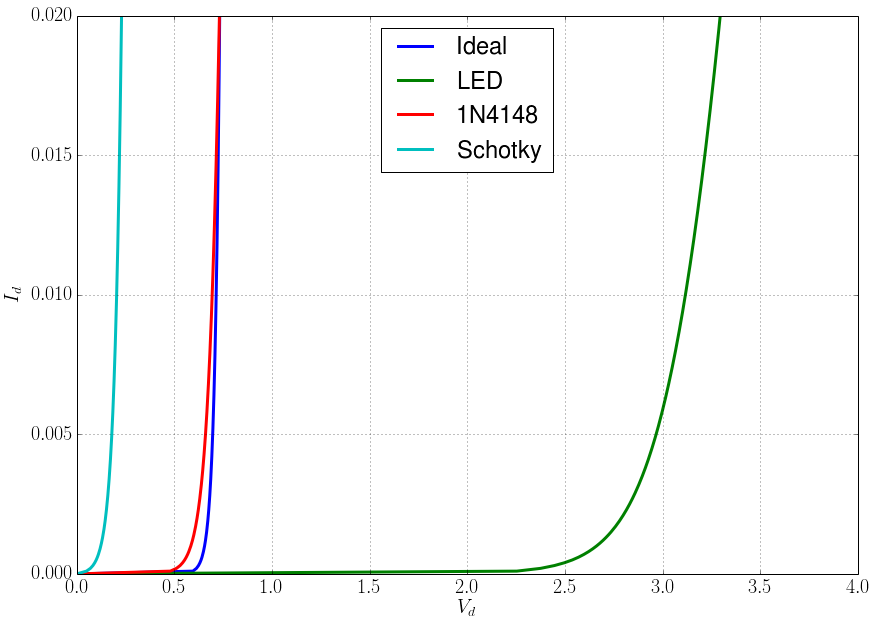
\includegraphics[max size={\textwidth}{\textheight}]{Graficar datos de ltspice_files/Graficar datos de ltspice_1_0.png}
    \par
    \end{center}
    
            \end{InvisibleVerbatim}
            
        
    


    % Make sure that atleast 4 lines are below the HR
    \needspace{4\baselineskip}

    
        \vspace{6pt}
        \makebox[0.1\linewidth]{\smaller\hfill\tt\color{nbframe-in-prompt}In\hspace{4pt}{[}24{]}:\hspace{4pt}}\\*
        \vspace{-2.65\baselineskip}
        \begin{ColorVerbatim}
            \vspace{-0.7\baselineskip}
            \begin{Verbatim}[commandchars=\\\{\}]
\PY{k+kn}{import} \PY{n+nn}{numpy} \PY{k+kn}{as} \PY{n+nn}{np}
\PY{k+kn}{import} \PY{n+nn}{pylab}
\PY{k+kn}{from} \PY{n+nn}{scipy.signal} \PY{k+kn}{import} \PY{n}{argrelextrema}

\PY{n}{filename} \PY{o}{=} \PY{l+s}{\PYZsq{}}\PY{l+s}{modulardoam[1].txt}\PY{l+s}{\PYZsq{}}

\PY{c}{\PYZsh{} Using the newer with construct to close the file automatically.}
\PY{k}{with} \PY{n+nb}{open}\PY{p}{(}\PY{n}{filename}\PY{p}{)} \PY{k}{as} \PY{n}{f}\PY{p}{:}
    \PY{n}{data} \PY{o}{=} \PY{n}{f}\PY{o}{.}\PY{n}{readlines}\PY{p}{(}\PY{p}{)}

\PY{n}{data2}\PY{o}{=}\PY{p}{[}\PY{p}{]}
\PY{k}{for} \PY{n}{i} \PY{o+ow}{in} \PY{n}{data}\PY{p}{[}\PY{l+m+mi}{1}\PY{p}{:}\PY{n+nb}{len}\PY{p}{(}\PY{n}{data}\PY{p}{)}\PY{p}{]}\PY{p}{:}
    \PY{n}{data2}\PY{o}{.}\PY{n}{append}\PY{p}{(}\PY{n}{i}\PY{o}{.}\PY{n}{strip}\PY{p}{(}\PY{p}{)}\PY{p}{)}
\end{Verbatim}

            
                \vspace{-0.2\baselineskip}
            
        \end{ColorVerbatim}
    


    % Make sure that atleast 4 lines are below the HR
    \needspace{4\baselineskip}

    
        \vspace{6pt}
        \makebox[0.1\linewidth]{\smaller\hfill\tt\color{nbframe-in-prompt}In\hspace{4pt}{[}3{]}:\hspace{4pt}}\\*
        \vspace{-2.65\baselineskip}
        \begin{ColorVerbatim}
            \vspace{-0.7\baselineskip}
            \begin{Verbatim}[commandchars=\\\{\}]
\PY{n}{t}\PY{o}{=}\PY{p}{[}\PY{p}{]}
\PY{n}{i1}\PY{o}{=}\PY{p}{[}\PY{p}{]}
\PY{n}{i2}\PY{o}{=}\PY{p}{[}\PY{p}{]}
\PY{k}{for} \PY{n}{i} \PY{o+ow}{in} \PY{n}{data2}\PY{p}{:}
    \PY{n}{s}\PY{o}{=}\PY{n}{i}\PY{o}{.}\PY{n}{split}\PY{p}{(}\PY{l+s}{\PYZsq{}}\PY{l+s+se}{\PYZbs{}t}\PY{l+s}{\PYZsq{}}\PY{p}{)}
    \PY{n}{t}\PY{o}{.}\PY{n}{append}\PY{p}{(}\PY{n}{s}\PY{p}{[}\PY{l+m+mi}{0}\PY{p}{]}\PY{p}{)}
    \PY{n}{i1}\PY{o}{.}\PY{n}{append}\PY{p}{(}\PY{n}{s}\PY{p}{[}\PY{l+m+mi}{1}\PY{p}{]}\PY{o}{.}\PY{n}{split}\PY{p}{(}\PY{l+s}{\PYZsq{}}\PY{l+s}{,}\PY{l+s}{\PYZsq{}}\PY{p}{)}\PY{p}{)}
    \PY{n}{i2}\PY{o}{.}\PY{n}{append}\PY{p}{(}\PY{n}{s}\PY{p}{[}\PY{l+m+mi}{2}\PY{p}{]}\PY{o}{.}\PY{n}{split}\PY{p}{(}\PY{l+s}{\PYZsq{}}\PY{l+s}{,}\PY{l+s}{\PYZsq{}}\PY{p}{)}\PY{p}{)}

\PY{n}{i2n}\PY{o}{=}\PY{n}{np}\PY{o}{.}\PY{n}{asarray}\PY{p}{(}\PY{n}{i2}\PY{p}{,}\PY{n}{dtype}\PY{o}{=}\PY{n}{np}\PY{o}{.}\PY{n}{float32}\PY{p}{)}   
\PY{n}{i1n}\PY{o}{=}\PY{n}{np}\PY{o}{.}\PY{n}{asarray}\PY{p}{(}\PY{n}{i1}\PY{p}{,}\PY{n}{dtype}\PY{o}{=}\PY{n}{np}\PY{o}{.}\PY{n}{float32}\PY{p}{)}   
\PY{n}{t}\PY{o}{=}\PY{n}{np}\PY{o}{.}\PY{n}{asarray}\PY{p}{(}\PY{n}{t}\PY{p}{,}\PY{n}{dtype}\PY{o}{=}\PY{n}{np}\PY{o}{.}\PY{n}{float}\PY{p}{)}  
\end{Verbatim}

            
                \vspace{-0.2\baselineskip}
            
        \end{ColorVerbatim}
    


    % Make sure that atleast 4 lines are below the HR
    \needspace{4\baselineskip}

    
        \vspace{6pt}
        \makebox[0.1\linewidth]{\smaller\hfill\tt\color{nbframe-in-prompt}In\hspace{4pt}{[}45{]}:\hspace{4pt}}\\*
        \vspace{-2.65\baselineskip}
        \begin{ColorVerbatim}
            \vspace{-0.7\baselineskip}
            \begin{Verbatim}[commandchars=\\\{\}]
\PY{n}{i1f}\PY{o}{=}\PY{n}{i1n}\PY{p}{[}\PY{p}{:}\PY{p}{,}\PY{l+m+mi}{1}\PY{p}{]}\PY{o}{+}\PY{l+m+mi}{1j}\PY{o}{*}\PY{n}{i1n}\PY{p}{[}\PY{p}{:}\PY{p}{,}\PY{l+m+mi}{0}\PY{p}{]}
\PY{n}{i2f}\PY{o}{=}\PY{n}{i2n}\PY{p}{[}\PY{p}{:}\PY{p}{,}\PY{l+m+mi}{1}\PY{p}{]}\PY{o}{+}\PY{l+m+mi}{1j}\PY{o}{*}\PY{n}{i2n}\PY{p}{[}\PY{p}{:}\PY{p}{,}\PY{l+m+mi}{0}\PY{p}{]}
\PY{n}{i1max}\PY{o}{=}\PY{n}{np}\PY{o}{.}\PY{n}{array}\PY{p}{(}\PY{p}{[}\PY{p}{]}\PY{p}{)}
\PY{n}{i2max}\PY{o}{=}\PY{n}{np}\PY{o}{.}\PY{n}{array}\PY{p}{(}\PY{p}{[}\PY{p}{]}\PY{p}{)}
\PY{n}{tmax}\PY{o}{=}\PY{n}{np}\PY{o}{.}\PY{n}{array}\PY{p}{(}\PY{p}{[}\PY{p}{]}\PY{p}{)}
\PY{k}{for} \PY{n}{i} \PY{o+ow}{in} \PY{n+nb}{range}\PY{p}{(}\PY{l+m+mi}{0}\PY{p}{,}\PY{n+nb}{len}\PY{p}{(}\PY{n}{t}\PY{p}{)}\PY{p}{)}\PY{p}{:}
    \PY{k}{if} \PY{l+m+mi}{20}\PY{o}{*}\PY{n}{np}\PY{o}{.}\PY{n}{log10}\PY{p}{(}\PY{n}{np}\PY{o}{.}\PY{n}{abs}\PY{p}{(}\PY{n}{i1f}\PY{p}{[}\PY{n}{i}\PY{p}{]}\PY{p}{)}\PY{p}{)} \PY{o}{\PYZgt{}} \PY{o}{\PYZhy{}}\PY{l+m+mi}{120}\PY{p}{:}
        \PY{n}{i1max}\PY{o}{=}\PY{n}{np}\PY{o}{.}\PY{n}{append}\PY{p}{(}\PY{n}{i1max}\PY{p}{,}\PY{n}{i1f}\PY{p}{[}\PY{n}{i}\PY{p}{]}\PY{p}{)}
        \PY{n}{i2max}\PY{o}{=}\PY{n}{np}\PY{o}{.}\PY{n}{append}\PY{p}{(}\PY{n}{i2max}\PY{p}{,}\PY{n}{i2f}\PY{p}{[}\PY{n}{i}\PY{p}{]}\PY{p}{)}
        \PY{n}{tmax}\PY{o}{=}\PY{n}{np}\PY{o}{.}\PY{n}{append}\PY{p}{(}\PY{n}{tmax}\PY{p}{,}\PY{n}{t}\PY{p}{[}\PY{n}{i}\PY{p}{]}\PY{p}{)}
\PY{n}{index}\PY{o}{=}\PY{n}{argrelextrema}\PY{p}{(}\PY{n}{np}\PY{o}{.}\PY{n}{abs}\PY{p}{(}\PY{n}{i1max}\PY{p}{)}\PY{p}{,} \PY{n}{np}\PY{o}{.}\PY{n}{greater}\PY{p}{)}
\PY{n}{indexm}\PY{o}{=}\PY{n}{np}\PY{o}{.}\PY{n}{argmax}\PY{p}{(}\PY{n}{np}\PY{o}{.}\PY{n}{abs}\PY{p}{(}\PY{n}{i1max}\PY{p}{)}\PY{p}{)}
\PY{n}{index2}\PY{o}{=}\PY{n}{argrelextrema}\PY{p}{(}\PY{n}{np}\PY{o}{.}\PY{n}{abs}\PY{p}{(}\PY{n}{i2max}\PY{p}{)}\PY{p}{,} \PY{n}{np}\PY{o}{.}\PY{n}{greater}\PY{p}{)}
\PY{n}{indexm2}\PY{o}{=}\PY{n}{np}\PY{o}{.}\PY{n}{argmax}\PY{p}{(}\PY{n}{np}\PY{o}{.}\PY{n}{abs}\PY{p}{(}\PY{n}{i2max}\PY{p}{)}\PY{p}{)}
\end{Verbatim}

            
                \vspace{-0.2\baselineskip}
            
        \end{ColorVerbatim}
    


    % Make sure that atleast 4 lines are below the HR
    \needspace{4\baselineskip}

    
        \vspace{6pt}
        \makebox[0.1\linewidth]{\smaller\hfill\tt\color{nbframe-in-prompt}In\hspace{4pt}{[}84{]}:\hspace{4pt}}\\*
        \vspace{-2.65\baselineskip}
        \begin{ColorVerbatim}
            \vspace{-0.7\baselineskip}
            \begin{Verbatim}[commandchars=\\\{\}]
\PY{n}{matplotlib}\PY{o}{.}\PY{n}{rcParams}\PY{o}{.}\PY{n}{update}\PY{p}{(}\PY{p}{\PYZob{}}\PY{l+s}{\PYZsq{}}\PY{l+s}{font.size}\PY{l+s}{\PYZsq{}}\PY{p}{:} \PY{l+m+mi}{20}\PY{p}{,}\PY{l+s}{\PYZsq{}}\PY{l+s}{text.usetex}\PY{l+s}{\PYZsq{}}\PY{p}{:} \PY{n+nb+bp}{True}\PY{p}{\PYZcb{}}\PY{p}{)}
\PY{n}{figure}\PY{p}{(}\PY{n}{figsize}\PY{o}{=}\PY{p}{(}\PY{l+m+mi}{14}\PY{p}{,}\PY{l+m+mi}{10}\PY{p}{)}\PY{p}{,} \PY{n}{dpi}\PY{o}{=}\PY{l+m+mi}{150}\PY{p}{)}
\PY{n}{xlim}\PY{p}{(}\PY{l+m+mi}{5}\PY{p}{,}\PY{l+m+mf}{1e5}\PY{p}{)}
\PY{n}{ylim}\PY{p}{(}\PY{o}{\PYZhy{}}\PY{l+m+mi}{180}\PY{p}{,}\PY{o}{\PYZhy{}}\PY{l+m+mi}{50}\PY{p}{)}
\PY{n}{xlabel}\PY{p}{(}\PY{l+s}{\PYZsq{}}\PY{l+s}{Frecuencia \PYZdl{}}\PY{l+s}{\PYZbs{}}\PY{l+s}{omega\PYZdl{}}\PY{l+s}{\PYZsq{}}\PY{p}{)}
\PY{n}{ylabel}\PY{p}{(}\PY{l+s}{\PYZsq{}}\PY{l+s}{Amplitu (dB)}\PY{l+s}{\PYZsq{}}\PY{p}{)}
\PY{n}{semilogx}\PY{p}{(}\PY{n}{tmax}\PY{p}{[}\PY{n}{index}\PY{p}{]}\PY{p}{,}\PY{l+m+mi}{20}\PY{o}{*}\PY{n}{np}\PY{o}{.}\PY{n}{log10}\PY{p}{(}\PY{n}{np}\PY{o}{.}\PY{n}{abs}\PY{p}{(}\PY{n}{i1max}\PY{p}{[}\PY{n}{index}\PY{p}{]}\PY{p}{)}\PY{p}{)}\PY{p}{,}\PY{l+s}{\PYZsq{}}\PY{l+s}{rx}\PY{l+s}{\PYZsq{}}\PY{p}{)}
\PY{n}{semilogx}\PY{p}{(}\PY{n}{tmax}\PY{p}{[}\PY{n}{index2}\PY{p}{]}\PY{p}{,}\PY{l+m+mi}{20}\PY{o}{*}\PY{n}{np}\PY{o}{.}\PY{n}{log10}\PY{p}{(}\PY{n}{np}\PY{o}{.}\PY{n}{abs}\PY{p}{(}\PY{n}{i2max}\PY{p}{[}\PY{n}{index2}\PY{p}{]}\PY{p}{)}\PY{p}{)}\PY{p}{,}\PY{l+s}{\PYZsq{}}\PY{l+s}{ko}\PY{l+s}{\PYZsq{}}\PY{p}{)}
\PY{n}{semilogx}\PY{p}{(}\PY{n}{t}\PY{p}{,}\PY{l+m+mi}{20}\PY{o}{*}\PY{n}{np}\PY{o}{.}\PY{n}{log10}\PY{p}{(}\PY{n}{np}\PY{o}{.}\PY{n}{abs}\PY{p}{(}\PY{n}{i1f}\PY{p}{)}\PY{p}{)}\PY{p}{)}
\PY{n}{semilogx}\PY{p}{(}\PY{n}{t}\PY{p}{,}\PY{l+m+mi}{20}\PY{o}{*}\PY{n}{np}\PY{o}{.}\PY{n}{log10}\PY{p}{(}\PY{n}{np}\PY{o}{.}\PY{n}{abs}\PY{p}{(}\PY{n}{i2f}\PY{p}{)}\PY{p}{)}\PY{p}{)}
\PY{n}{annotate}\PY{p}{(}\PY{n+nb}{str}\PY{p}{(}\PY{n}{tmax}\PY{p}{[}\PY{n}{indexm}\PY{p}{]}\PY{p}{)}\PY{o}{+}\PY{l+s}{\PYZsq{}}\PY{l+s}{,}\PY{l+s}{\PYZsq{}}\PY{o}{+}\PY{n+nb}{str}\PY{p}{(}\PY{n+nb}{round}\PY{p}{(}\PY{l+m+mi}{20}\PY{o}{*}\PY{n}{np}\PY{o}{.}\PY{n}{log10}\PY{p}{(}\PY{n}{np}\PY{o}{.}\PY{n}{abs}\PY{p}{(}\PY{n}{i1max}\PY{p}{[}\PY{n}{indexm}\PY{p}{]}\PY{p}{)}\PY{p}{)}\PY{p}{,}\PY{l+m+mi}{2}\PY{p}{)}\PY{p}{)}\PY{p}{,} 
         \PY{n}{xy}\PY{o}{=}\PY{p}{(}\PY{n}{tmax}\PY{p}{[}\PY{n}{indexm}\PY{p}{]}\PY{p}{,}\PY{l+m+mi}{20}\PY{o}{*}\PY{n}{np}\PY{o}{.}\PY{n}{log10}\PY{p}{(}\PY{n}{np}\PY{o}{.}\PY{n}{abs}\PY{p}{(}\PY{n}{i1max}\PY{p}{[}\PY{n}{indexm}\PY{p}{]}\PY{p}{)}\PY{p}{)}\PY{p}{)}\PY{p}{,}
         \PY{n}{xycoords}\PY{o}{=}\PY{l+s}{\PYZsq{}}\PY{l+s}{data}\PY{l+s}{\PYZsq{}}\PY{p}{,}\PY{n}{xytext}\PY{o}{=}\PY{p}{(}\PY{o}{\PYZhy{}}\PY{l+m+mi}{100}\PY{p}{,} \PY{l+m+mi}{20}\PY{p}{)}\PY{p}{,} \PY{n}{textcoords}\PY{o}{=}\PY{l+s}{\PYZsq{}}\PY{l+s}{offset points}\PY{l+s}{\PYZsq{}}\PY{p}{,}
         \PY{n}{arrowprops}\PY{o}{=}\PY{n+nb}{dict}\PY{p}{(}\PY{n}{arrowstyle}\PY{o}{=}\PY{l+s}{\PYZdq{}}\PY{l+s}{\PYZhy{}\PYZgt{}}\PY{l+s}{\PYZdq{}}\PY{p}{,}\PY{n}{connectionstyle}\PY{o}{=}\PY{l+s}{\PYZdq{}}\PY{l+s}{arc3,rad=.2}\PY{l+s}{\PYZdq{}}\PY{p}{)}\PY{p}{,}
         \PY{n}{color} \PY{o}{=} \PY{l+s}{\PYZsq{}}\PY{l+s}{\PYZsh{}0000ee}\PY{l+s}{\PYZsq{}}\PY{p}{)}
\PY{n}{annotate}\PY{p}{(}\PY{l+s}{\PYZsq{}}\PY{l+s}{Primer maximo }\PY{l+s+se}{\PYZbs{}n}\PY{l+s}{\PYZsq{}}\PY{o}{+}\PY{n+nb}{str}\PY{p}{(}\PY{n}{tmax}\PY{p}{[}\PY{l+m+mi}{1}\PY{p}{]}\PY{p}{)}\PY{o}{+}\PY{l+s}{\PYZsq{}}\PY{l+s}{,}\PY{l+s}{\PYZsq{}}\PY{o}{+}\PY{n+nb}{str}\PY{p}{(}\PY{n+nb}{round}\PY{p}{(}\PY{l+m+mi}{20}\PY{o}{*}\PY{n}{np}\PY{o}{.}\PY{n}{log10}\PY{p}{(}\PY{n}{np}\PY{o}{.}\PY{n}{abs}\PY{p}{(}\PY{n}{i1max}\PY{p}{[}\PY{l+m+mi}{1}\PY{p}{]}\PY{p}{)}\PY{p}{)}\PY{p}{,}\PY{l+m+mi}{2}\PY{p}{)}\PY{p}{)}\PY{p}{,}
         \PY{n}{xy}\PY{o}{=}\PY{p}{(}\PY{n}{tmax}\PY{p}{[}\PY{l+m+mi}{1}\PY{p}{]}\PY{p}{,}\PY{l+m+mi}{20}\PY{o}{*}\PY{n}{np}\PY{o}{.}\PY{n}{log10}\PY{p}{(}\PY{n}{np}\PY{o}{.}\PY{n}{abs}\PY{p}{(}\PY{n}{i1max}\PY{p}{[}\PY{l+m+mi}{1}\PY{p}{]}\PY{p}{)}\PY{p}{)}\PY{p}{)}\PY{p}{,}  \PY{n}{xycoords}\PY{o}{=}\PY{l+s}{\PYZsq{}}\PY{l+s}{data}\PY{l+s}{\PYZsq{}}\PY{p}{,}\PY{n}{xytext}\PY{o}{=}\PY{p}{(}\PY{o}{\PYZhy{}}\PY{l+m+mi}{70}\PY{p}{,} \PY{l+m+mi}{40}\PY{p}{)}\PY{p}{,}
         \PY{n}{textcoords}\PY{o}{=}\PY{l+s}{\PYZsq{}}\PY{l+s}{offset points}\PY{l+s}{\PYZsq{}}\PY{p}{,}\PY{n}{arrowprops}\PY{o}{=}\PY{n+nb}{dict}\PY{p}{(}\PY{n}{arrowstyle}\PY{o}{=}\PY{l+s}{\PYZdq{}}\PY{l+s}{\PYZhy{}\PYZgt{}}\PY{l+s}{\PYZdq{}}\PY{p}{,}\PY{n}{connectionstyle}\PY{o}{=}\PY{l+s}{\PYZdq{}}\PY{l+s}{arc3,rad=.2}\PY{l+s}{\PYZdq{}}\PY{p}{)}\PY{p}{,}
         \PY{n}{color} \PY{o}{=} \PY{l+s}{\PYZsq{}}\PY{l+s}{\PYZsh{}0000ee}\PY{l+s}{\PYZsq{}}\PY{p}{)}
\PY{n}{annotate}\PY{p}{(}\PY{l+s}{\PYZsq{}}\PY{l+s}{Primer maximo }\PY{l+s+se}{\PYZbs{}n}\PY{l+s}{\PYZsq{}}\PY{o}{+}\PY{n+nb}{str}\PY{p}{(}\PY{n}{tmax}\PY{p}{[}\PY{n}{indexm2}\PY{p}{]}\PY{p}{)}\PY{o}{+}\PY{l+s}{\PYZsq{}}\PY{l+s}{,}\PY{l+s}{\PYZsq{}}\PY{o}{+}\PY{n+nb}{str}\PY{p}{(}\PY{n+nb}{round}\PY{p}{(}\PY{l+m+mi}{20}\PY{o}{*}\PY{n}{np}\PY{o}{.}\PY{n}{log10}\PY{p}{(}\PY{n}{np}\PY{o}{.}\PY{n}{abs}\PY{p}{(}\PY{n}{i2max}\PY{p}{[}\PY{n}{indexm2}\PY{p}{]}\PY{p}{)}\PY{p}{)}\PY{p}{,}\PY{l+m+mi}{2}\PY{p}{)}\PY{p}{)}\PY{p}{,} 
         \PY{n}{xy}\PY{o}{=}\PY{p}{(}\PY{n}{tmax}\PY{p}{[}\PY{n}{indexm2}\PY{p}{]}\PY{p}{,}\PY{l+m+mi}{20}\PY{o}{*}\PY{n}{np}\PY{o}{.}\PY{n}{log10}\PY{p}{(}\PY{n}{np}\PY{o}{.}\PY{n}{abs}\PY{p}{(}\PY{n}{i2max}\PY{p}{[}\PY{n}{indexm2}\PY{p}{]}\PY{p}{)}\PY{p}{)}\PY{p}{)}\PY{p}{,}
         \PY{n}{xycoords}\PY{o}{=}\PY{l+s}{\PYZsq{}}\PY{l+s}{data}\PY{l+s}{\PYZsq{}}\PY{p}{,}\PY{n}{xytext}\PY{o}{=}\PY{p}{(}\PY{l+m+mi}{50}\PY{p}{,} \PY{l+m+mi}{20}\PY{p}{)}\PY{p}{,} \PY{n}{textcoords}\PY{o}{=}\PY{l+s}{\PYZsq{}}\PY{l+s}{offset points}\PY{l+s}{\PYZsq{}}\PY{p}{,}
         \PY{n}{arrowprops}\PY{o}{=}\PY{n+nb}{dict}\PY{p}{(}\PY{n}{arrowstyle}\PY{o}{=}\PY{l+s}{\PYZdq{}}\PY{l+s}{\PYZhy{}\PYZgt{}}\PY{l+s}{\PYZdq{}}\PY{p}{,}\PY{n}{connectionstyle}\PY{o}{=}\PY{l+s}{\PYZdq{}}\PY{l+s}{arc3,rad=.2}\PY{l+s}{\PYZdq{}}\PY{p}{)}\PY{p}{,}
         \PY{n}{color} \PY{o}{=} \PY{l+s}{\PYZsq{}}\PY{l+s}{\PYZsh{}009900}\PY{l+s}{\PYZsq{}}\PY{p}{)}
\PY{n}{grid}\PY{p}{(}\PY{p}{)}
\PY{n}{savefig}\PY{p}{(}\PY{l+s}{\PYZsq{}}\PY{l+s}{images/espectroam.png}\PY{l+s}{\PYZsq{}}\PY{p}{)}
\end{Verbatim}

            
                \vspace{-0.2\baselineskip}
            
        \end{ColorVerbatim}
    

    

        % If the first block is an image, minipage the image.  Else
        % request a certain amount of space for the input text.
        \needspace{4\baselineskip}
        
        

            % Add document contents.
            
                \begin{InvisibleVerbatim}
                \vspace{-0.5\baselineskip}
    \begin{center}
    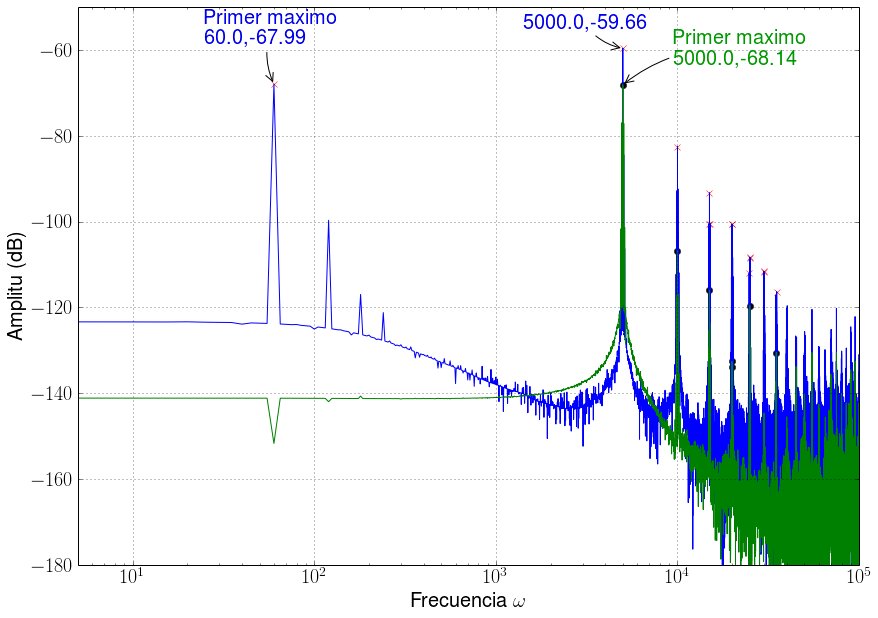
\includegraphics[max size={\textwidth}{\textheight}]{Graficar datos de ltspice_files/Graficar datos de ltspice_5_0.png}
    \par
    \end{center}
    
            \end{InvisibleVerbatim}
            
        
    


    % Make sure that atleast 4 lines are below the HR
    \needspace{4\baselineskip}

    
        \vspace{6pt}
        \makebox[0.1\linewidth]{\smaller\hfill\tt\color{nbframe-in-prompt}In\hspace{4pt}{[}{]}:\hspace{4pt}}\\*
        \vspace{-2.65\baselineskip}
        \begin{ColorVerbatim}
            \vspace{-0.7\baselineskip}
            \begin{Verbatim}[commandchars=\\\{\}]

\end{Verbatim}

            
                \vspace{0.3\baselineskip}
            
        \end{ColorVerbatim}
    

        

        \renewcommand{\indexname}{Index}
        \printindex

    % End of document
    \end{document}


